% Kapitel 3: Hardware- und Technologieauswahl
\section{Hardware- und Technologieauswahl}
\label{sec:hardware}

\subsection{Hardwareauswahl}

Die Auswahl der Hardware ist entscheidend für die Zuverlässigkeit und Präzision der Kennzeichenerkennung und des Gesamtsystems.
Diese beschränkt sich für diese Diplomarbeit auf zwei primäre Komponenten:
Einerseits wird eine Kamera benötigt, welche Live-Daten von der Ein- und Ausfahrt des Parkplatzes erfasst und diese weitersenden kann.
Zudem ein Server oder ähnliches, auf dem die Services der Diplomarbeit deployed werden können, und welcher für die rechenintensiven Aufgaben zuständig ist.

Das folgende Kapitel soll einen Einblick in den Entscheidungsprozess bieten, nach dem die benötigte Hardware ausgewählt wurde.
Hierfür werden zunächst die Grundanforderungen an das Gesamtsystem aus der Aufgabenstellung (Abschnitt~\ref{sec:aufgabenstellung}) abgeleitet, darauf aufbauend werden dann die spezifischen Anforderungen an die Hardwarekomponenten dargelegt.
Danach werden die einzelnen, im Auswahlprozess evaluierten Optionen gegenübergestellt und hinsichtlich ihrer Eignung analysiert.

\begin{figure}[htbp]
    \centering
    
\includegraphics[width=\textwidth]{zotter.png}
    \caption{Luftbild des Hauptgebäudes und Parkplatz der Zotter Schokolade GmbH}
    \source{Google, Google Earth: \url{https://earth.google.com/}}
    \label{fig:zotter_luftbild}
\end{figure}

\newpage
\subsubsection{Anforderungsanalyse an die Hardware}

\paragraph{Grundanforderungen}
Wie oben kurz erwähnt, existieren einige Anforderungen, welche für die Funktionsfähigkeit des Systems unausweichlich sind.
Zunächst galt es, die Gegebenheiten vor Ort zu betrachten, also Lage und Aufbau des Bereiches, in dem der Fahrzeugverkehr erkannt werden sollte.

Wie das Luftbild (Abb. \ref{fig:zotter_luftbild}) zeigt, verfügt der Parkplatz über eine kombinierte Ein- und Ausfahrt.
Dies reduziert zwar den Installationsaufwand der Hardware, erhöht jedoch die Software-Komplexität, da die Bewegungsrichtung der Fahrzeuge softwareseitig erkannt werden muss.
Das Zeitintervall zwischen zwei aufeinanderfolgenden Fahrzeugen wurde aufgrund der Breite der Einfahrt auf zwei bis drei Sekunden geschätzt.
Das System sollte folglich in der Lage sein, 20 bis 30 Bilder pro Minute zu analysieren und die daraus gewonnenen Daten persistent zu speichern.

\paragraph{Anforderungen Kamera}
Da die Kamera im Außenbereich eingesetzt wird, ist eine gewisse Witterungsbeständigkeit zwingend erforderlich.
Aufgrund der notwendigen Positionierung der Kamera sollte diese mindestens die Schutzklasse IP66 (Ingress Protection) erfüllen,
was einem Schutz vor starken Wasserstrahlen aus allen Richtungen entspricht. \cite{baseus_ip_ratings}

Da das Kennzeichenerkennungssystem primär für die Erfassung von Kunden-Kennzeichen konzipiert ist, ist von einer effektiven Hauptbetriebszeit während der Öffnungszeiten der Zotter-Erlebniswelt ausgegangen worden.
Diese betragen: Mo--Fr: 9--18 Uhr, Sa: 9--18:30 Uhr.
Aufgrund dessen lag im Entscheidungsprozess kein großes Augenmerk auf den Nachtsichtfähigkeiten des Kamerasystems.

\paragraph{Anforderungen Server}
Die notwendige Rechenleistung des Servers hängt sehr stark von der Komplexität und Art der Prozesse ab, welche auf diesem ausgerollt und aktiv sind.
Deshalb wurde diese anfangs absichtlich nicht genau definiert.
Festgelegt wurde jedoch der Einsatz eines Linux-Betriebssystems, da dieses dem internen Unternehmensstandard entspricht, einen geringen OS-Overhead aufweist und eine breite Kompatibilität bietet.
Dies wurde allerdings als zweitrangig betrachtet, da das System durch die Verwendung von Containerisierung mit Docker ohnehin eine Plattformunabhängigkeit bietet.
Auch wurde seitens Zotter vorausgesetzt, dass sämtliche Daten nicht nur aus Datenschutzgründen On-Premise, sondern für eine bessere Isolation des Systems lokal auf dem eingesetzten Server gespeichert werden sollen.


\subsubsection{Evaluierung der Hardware-Optionen}

\paragraph{Kamera -- Auswahl}

In Bezug auf die Kamera wurden von Anfang an nur IP-Kameras in Betracht gezogen, also Kameras, bei denen Video-Streams und Kommunikation per Ethernet stattfinden.
Dies hat zwei Hauptgründe:
Daten können zunächst in den meisten Fällen direkt per API-Requests ausgelesen werden, entweder über HTTP/REST-APIs oder im Fall von Video-Streams über RTSP (Real Time Streaming Protocol).
Zudem nutzen viele IP-Kameras PoE (Power over Ethernet) für ihre Spannungsversorgung, was die Aufbaukomplexität weiter minimiert, da nur ein Kabel, welches Strom und Daten überträgt, verlegt werden muss. \cite{wiki_ip_camera}

Vor dem offiziellen Start der Diplomarbeit wurden hierzu schon einige Überlegungen angestellt und mögliche Produkt-Kandidaten vorgemerkt.
Im Zuge von Gesprächen mit Michael Zotter wurde darauf aufmerksam gemacht, dass bereits einige IP-Kameras des Herstellers Synology für frühere Testversuche angeschafft wurden.
Besonders das Modell BC500, von welchem einige Stück bereits im Besitz der Firma Zotter waren, erschien als besonders geeignet. \cite{synology_bc500}

\begin{figure}[htbp]
    \centering
    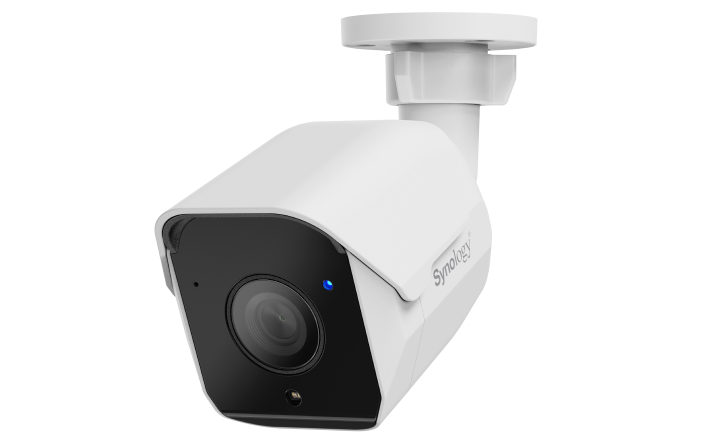
\includegraphics[width=8cm]{synology_bc500.png}
    \caption{Synology BC500}
    \source{\url{https://fileres.synology.com/images/ec/products/BC500.jpg}}
    \label{fig:synology_bc500}
\end{figure}

Mit einer Witterungsbeständigkeitsbewertung von IP67, da als Außenkamera konzipiert, ist diese gut für den Außeneinsatz geeignet.
Die maximale Videoauflösung von 2880$\times$1620 Pixel bei maximal 30 FPS erschien auch für eine konsistente Kennzeichenerkennung ausreichend.
Auch verfügt die BC500 über eine automatische Nachtsichtfunktion mittels Infrarot-LEDs.
Zusätzlich schien die BC500 über eine robuste API für das Auslesen von Daten und das Streamen des Feeds zu verfügen.

Aufgrund der oben angesprochenen sofortigen Verfügbarkeit und des wegfallenden Mehraufwands für diese Kamera, verbunden mit den genannten Spezifikationen, fiel die Entscheidung nach Absprache mit unserer Kontaktperson auf das Synology-Modell.

\newpage
\paragraph{Kamera -- Montage}

Das Kamerasystem wurde, wie unten erkenntlich (Abb. \ref{fig:kamera_montage}), so montiert, dass es in Richtung des Parkplatzes zeigt.
Dies erwies sich als die optimale Wahl, da so der mögliche Erkennungsbereich maximiert wird und die Montage an dieser Position einfacher realisierbar war.
Bei der genauen Positionierung und Ausrichtung der Kamera wurde versucht, sich so gut wie möglich am Kamera-Setup-Guide von Plate Recognizer zu orientieren. \cite{platerecognizer_camera_setup}

Die erforderliche Netzwerkverkabelung wurde, wie oben im Bild ersichtlich, über den bereits vorhandenen Kabelkanal der Sicherheitsschranke geführt.
Dieser verläuft bis in den Netzwerkschrank im angrenzenden Bürogebäude, wo die Anbindung an das Firmennetzwerk erfolgt.

\begin{figure}[htbp]
    \centering
    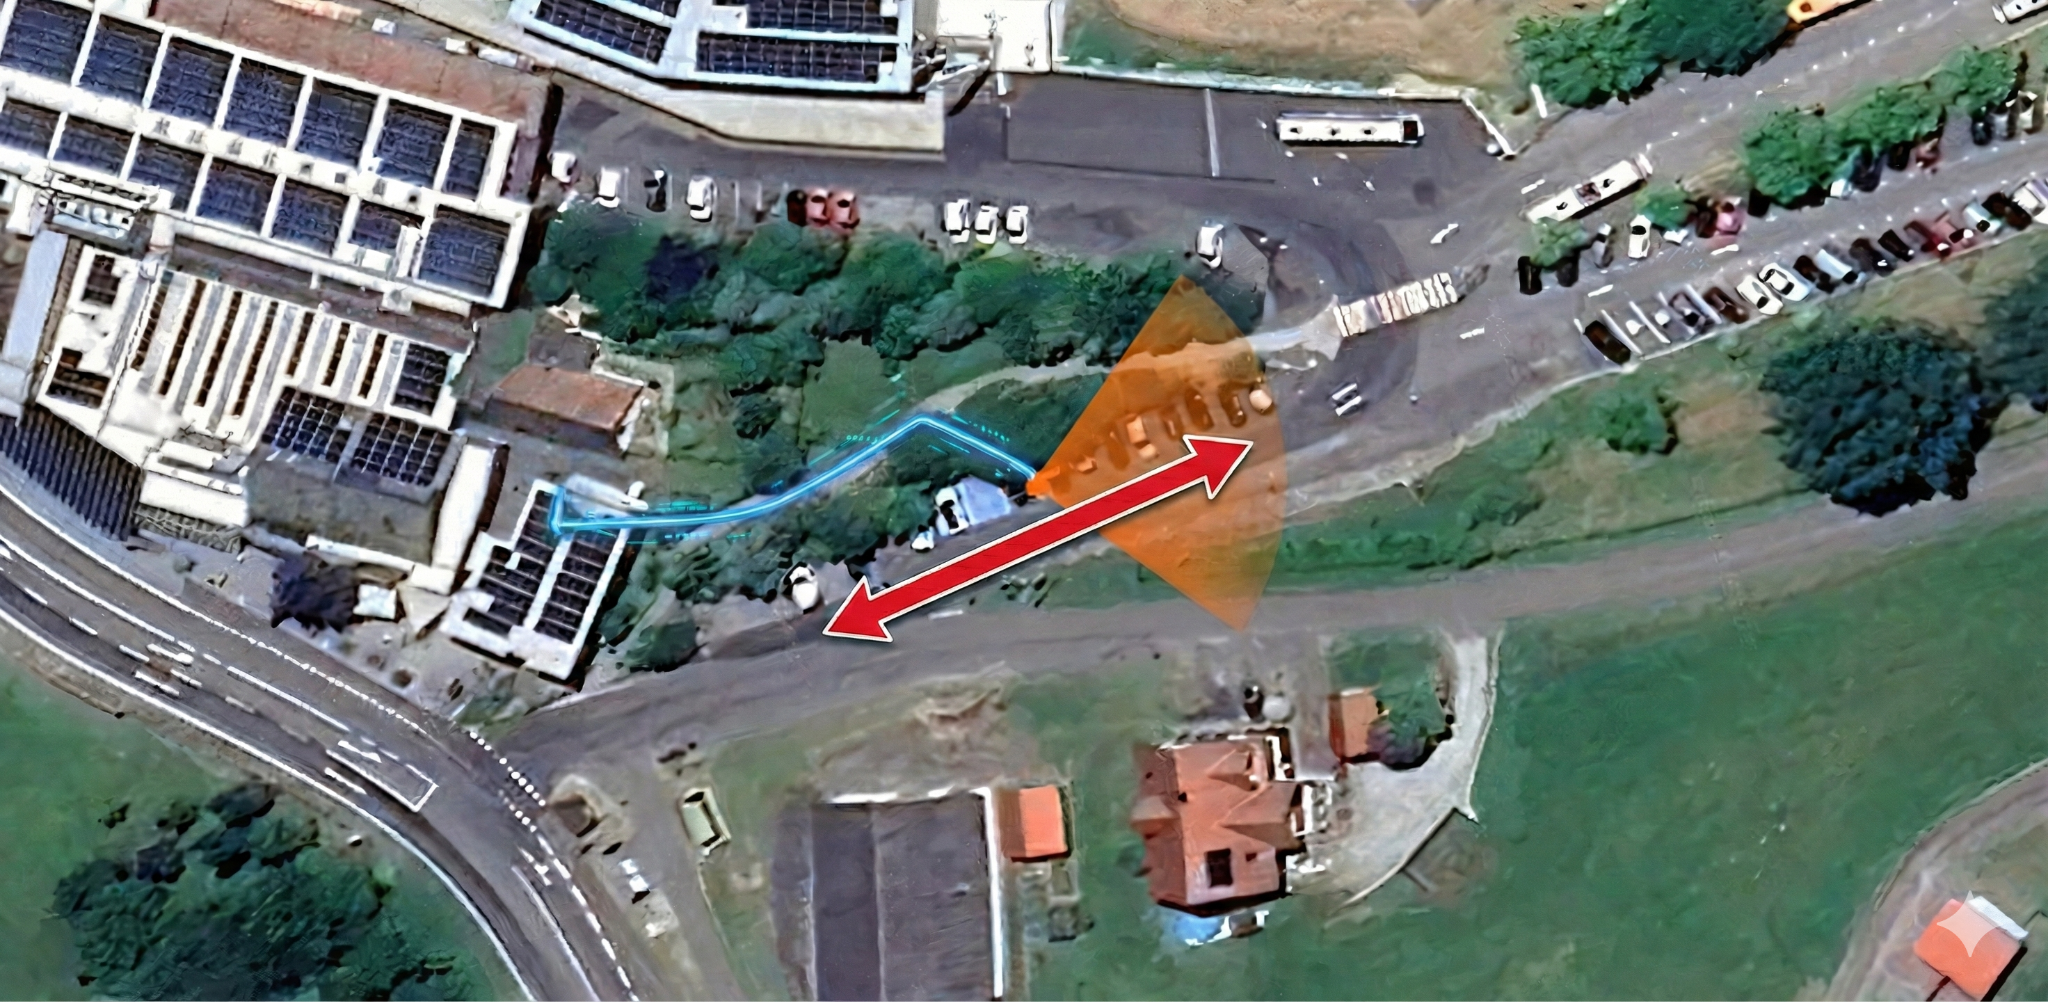
\includegraphics[width=\textwidth]{zotter-markup.png}
    \caption{Markup der Kamerapositionierung}
    \source{Google, Google Earth: \url{https://earth.google.com/}}
    \label{fig:kamera_montage}
\end{figure}

\newpage
\paragraph{Server -- Auswahl}

Die gewählte Microservice-Architektur im Zusammenspiel mit der angewandten Containerisierung erlaubt eine hohe Flexibilität für die Art der benötigten Hardware.
Des Weiteren war aus einem früheren Praktikum bei Zotter Schokolade bekannt, dass die hausinterne Infrastruktur Kapazitäten für Container-Deployment bietet.

Als zweite Option wurde das Einrichten eines kleinen Servers auf der Hardware eines Office-Mini-PCs erwogen.
Dieser wäre aus reiner Implementierungs- und Funktionssicht mit der ersten Option gleichwertig, mit dem Vorteil, dass dieser Ansatz eine gewisse Unabhängigkeit zum internen Netzwerk und zur zentralen Infrastruktur ermöglicht.

An diesem Punkt wurde im Kamera-Entscheidungsprozess auf die bestehenden Synology-Produkte aufmerksam gemacht.
Mit dieser Neuausrichtung kam die Idee auf, das System auf einem eigenen NAS-System (Network-attached Storage), ebenfalls von Synology zu betreiben.

Nicht nur wurden NAS-Systeme von Synology bereits im Unternehmen eingesetzt, diese sind in den meisten Bereichen gleichwertig mit den vorherigen beiden diskutierten Ansätzen und bieten in manchen Bereichen klare Vorteile \cite{aws_nas}:
\begin{enumerate}
    \item Die Vorteile der zweiten Option bleiben bestehen, es gibt weiterhin eine gesteigerte Unabhängigkeit zur Unternehmensinfrastruktur und damit hergehend mehr Entwicklungsfreiheit.
    \item Da es sich um ein NAS-System handelt, also ein Gerät, welches primär für die Speicherung von Daten konzipiert ist, stellt der benötigte Speicherplatz kein Problem mehr dar, da einfach neue Disks verbaut werden können (z.B. 2$\times$ 2TB Disks, RAID 1).
    \item Diese NAS-Systeme besitzen bereits leistungsstarke Komponenten, welche in Bezug auf Rechenleistung meist gleichwertig zu einem durchschnittlichen Mini-PC sind.
          Auch sind die meisten NAS-Geräte mit einem vollwertigen Betriebssystem ausgestattet, welches Methoden bereitstellt, um Container mittels Docker reibungslos laufen zu lassen.
\end{enumerate}

Der größte Vorteil kommt aber mit der Kombination mit den oben beschriebenen Kameras des gleichnamigen Herstellers.
Wie die Kameralinie von Synology vermuten lässt, bietet der Hersteller eigene Produkte gezielt für Überwachungsaufgaben an.
Diese laufen unter einem Gesamtsystem mit der Bezeichnung "`Surveillance Station"' und sind als Paket auf den hauseigenen NAS-Systemen verfügbar. \cite{synology_surveillance}

\newpage
Innerhalb des Surveillance Station-Ökosystems bietet Synology mit der DVA-Serie (Deep Video Analytics) spezialisierte NVR-Geräte (Network Video Recorder) an, welche über GPU-beschleunigte KI-Funktionen verfügen.
Insbesondere das Modell DVA1622 (zur Zeit des Projekts das einzige verfügbare Modell der DVA-Serie) bietet für diese Diplomarbeit in Kombination mit der Kamera BC500 viele Vorteile: \cite{synology_dva}

\begin{figure}[htbp]
    \centering
    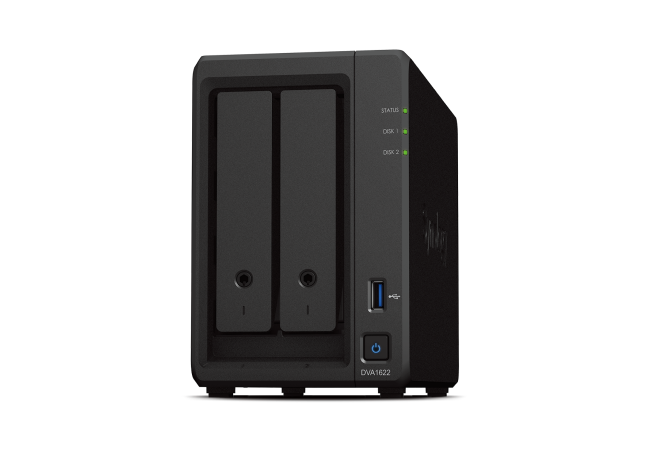
\includegraphics[width=8cm]{synology_dva1622.png}
    \caption{Synology DVA1622}
    \source{\url{https://www.synology.com/img/products/detail/DVA1622/heading.png}}
    \label{fig:synology_dva1622}
\end{figure}

Zunächst bietet die Surveillance Station API Zugriff auf Live-Streams, Snapshots und Ereignis-Metadaten, was die Integration in eigene Microservices im Vergleich zum direkten Auslesen aus Kameras erheblich vereinfacht.
Die DVA-Serie unterstützt nativ viele Features aus dem Security- und Surveillance-Bereich.
So können etwa mittels Erkennungszonen bereits auf Surveillance Station-Ebene relevante Bildbereiche wie der Einfahrtsbereich definiert werden. \cite{synology_dva}
Dies ist besonders für das Erstellen von "`Triggers"' relevant, also das Anlegen eines Bereiches, in dem im Falle einer Fahrzeugdurchfahrt die Kennzeichenerkennung stattfinden soll.
Des Weiteren können alle Kamera-Einstellungen, Aufzeichnungen und Analysen über eine einheitliche Oberfläche auf dem NAS-Gerät verwaltet werden. \cite{synology_surveillance}

Die Kombination aus relevanten Features, umfassender API und nativer Kamera-Unterstützung machte das Synology DVA1622-NAS zur optimalen Wahl für die Realisierung des Kennzeichenerkennungssystems.


\paragraph{Server -- Montage}

Das NAS-System ist durch seine Kompaktheit und Kapselung auf keine besonderen Anforderungen an den Montage- bzw. Betriebsort angewiesen.
Aus diesem Grund wurde dieses innerhalb des Bürogebäudes installiert, in welchem auch die Kamera an das Firmennetzwerk angeschlossen ist.

\newpage
\subsection{Technik-Stack und Technologieauswahl der Kennzeichenerkennung}
\label{sec:techstack}

\subsubsection{Technologieauswahl Kennzeichenerkennung}

Für die eigentliche Kennzeichenerkennung stand die Entscheidung zwischen der Entwicklung einer eigenen Lösung auf Basis von Open-Source-OCR-Bibliotheken (wie Tesseract OCR oder EasyOCR) und der Verwendung einer kommerziellen Lösung im Raum.

Bei der Evaluation von Tesseract und EasyOCR zeigte sich, dass diese generischen OCR-Engines zwar für Texterkennungsaufgaben gut geeignet sind, bei der spezifischen Herausforderung der Kennzeichenerkennung jedoch erhebliche Nachteile aufweisen.
Kennzeichen stellen besondere Anforderungen an ein Erkennungssystem, wie im Kapitel~\ref{sec:alpr} bereits erwähnt:
Sie müssen aus verschiedenen Winkeln, bei unterschiedlichen Lichtverhältnissen, mit Verschmutzungen und in Bewegung zuverlässig erkannt werden.
Zudem variieren Kennzeichenformate international stark in Schriftart, Layout und Zeichenabständen.

Als weitere Option wurde die Verwendung der Synology-nativen Lösung zur Kennzeichenerkennung erwogen.
Dies erwies sich aber schnell als nicht umsetzbar, da die Erkennung laut Hersteller auf dem Modell DVA1622 nur für stationäre Fahrzeuge ausgelegt ist. \cite{synology_lpr}

Die Entwicklung eines eigenen trainierten Modells auf Basis dieser Bibliotheken hätte einen erheblichen Aufwand für das Sammeln und Annotieren von Trainingsdaten bedeutet, wobei die resultierende Genauigkeit dennoch fraglich geblieben wäre.
In diese Richtung wurden im Zuge der Diplomarbeit-Entwicklung Prototypen erstellt, diese blieben aber in ihrer Qualität unzureichend oder waren in ihrem Realisierungsaufwand unrealistisch.

Aus diesem Grund fiel die Entscheidung auf Plate Recognizer, eine spezialisierte kommerzielle Lösung für Kennzeichenerkennung.
Plate Recognizer bietet hochoptimierte Machine-Learning-Modelle, welche bereits auf Kennzeichenbildern aus über 90 Ländern trainiert wurden. \cite{platerecognizer_countries}
Dies gewährleistet eine deutlich höhere Erkennungsrate auch unter erschwerten Bedingungen \cite{platerecognizer_results}.
Wie im Kapitel~\ref{sec:mmc} erwähnt bietet diese Lösung, zusätzlich zur reinen Texterkennung, erweiterte Funktionen wie Fahrzeugtyp- und Farberkennung, welche für zukünftige Erweiterungen des Systems nützlich sein können.

Ein weiterer entscheidender Vorteil ist die Verfügbarkeit als Docker-Container (Plate Recognizer SDK), der vollständig lokal auf dem DVA1622 NAS betrieben werden kann.
Im Gegensatz zu Cloud-basierten API-Lösungen bleiben damit alle Bilddaten im lokalen Netzwerk, was sowohl Datenschutzanforderungen erfüllt als auch Latenzzeiten minimiert. \cite{platerecognizer_snapshot}


\subsubsection{Argumentation der Software-Technologien Entscheidungen}

Als Web-Framework wurde FastAPI auf Python gewählt \cite{fastapi}, welches moderne asynchrone Request-Verarbeitung unterstützt und automatische API-Dokumentation via OpenAPI/Swagger generiert.
Im Vergleich zu Flask, dem vermutlich bekanntesten Python-Framework, bietet FastAPI native Type-Hints-Unterstützung und automatische Validierung von Request-/Response-Daten durch Pydantic. \cite{jetbrains_frameworks}
Gegenüber dem schwergewichtigeren Django bringt FastAPI deutlich weniger Overhead mit und ist damit besser für kleine Microservices geeignet, bei denen schlanke, spezialisierte Services bevorzugt werden. \cite{jetbrains_frameworks}

Für die Datenhaltung wurde PostgreSQL als relationale Datenbank gewählt. \cite{postgresql}
Während NoSQL-Datenbanken wie MongoDB für hochskalierbare, dokumentenbasierte Anwendungen Vorteile bieten, sprechen im vorliegenden Fall die strukturierten Datenbeziehungen (Erkennungen, Benutzer etc.) klar für eine relationale Datenbank.

Um Datenbank-Schema Änderungen versioniert und reproduzierbar zu gestalten, wurde Alembic als Migrations-Framework gewählt \cite{alembic}.
Im Gegensatz zu manuellen SQL-Skripten ermöglicht dies rückverfolgbare Datenbankänderungen, die automatisiert über alle Umgebungen ausgerollt werden können.

Das Gesamtsystem basiert auf Docker und einer Microservice-Architektur.
Wie zuvor detailliert erklärt, läuft jeder Dienst (Data Collection, Notification, Grafana) in seinem eigenen Container mit klar definierten Schnittstellen.
Dies verhindert wie in den Theoretischen Grundlagen erklärt nicht nur Abhängigkeitskonflikte zwischen verschiedenen Services, sondern ermöglicht auch die unabhängige Skalierung einzelner Komponenten.
Die Containerisierung gewährleistet zudem Plattformunabhängigkeit, da das System problemlos von der Synology-Plattform auf andere migriert werden kann, ohne dass Anpassungen am Code notwendig sind.
